\documentclass{article}
\usepackage[utf8]{inputenc}

\usepackage[letterpaper, margin=1in]{geometry}
\title{Reinforcement Learning}
\author{Mihir Patel}
\date{March 2018}

\usepackage{natbib}
\usepackage{graphicx}
\usepackage{amsmath}
\usepackage{sidecap}

\begin{document}

\maketitle

\section{Introduction}
\label{submission}

With the advent of graphical processing units (GPUs) and tensor processing units (TPUs), machine and deep learning has played a key role in the flurry of artificial intelligence advancements. Yet while great progress has been made in perception tasks like natural language processing and image analysis, improvements in logic and decision making have been relatively slow. This is primarily because deep learning requires high volumes of data that are well annotated.

Perception is relatively well suited for this approach as data is easy to annotate and the correlation between the input, such as an image and the object classification, is not too distant. By contrast, vanilla supervised learning is not feasible for most decision making processes. For example, in a given game of chess, player A beats player B yet player B plays a far superior game with the exception of one critical mistake. If the win result was used to assign labels, most moves would be mislabeled. Assigning labels for deep learning is difficult, noisy, and often prone to error.

The primary way deep learning is applied to these problems in a manner that resolves these issues is through reinforcement learning, which has achieved near miraculous results and bested both previous algorithms and human performance records across a variety of benchmarks. However, this technique is notoriously slow and computationally expensive.

\subsection{Markov Decision Processes}

At its core, decision making AI seek to model the function $f(state) = action$. They seek to extract information from a particular state and move in the most optimal manner possible from that state. In trivial cases, this can be brute-forced and hashed. However, in the vast majority of cases the state-space is very large, and it is too memory intensive to learn and record the optimal move for each state.

To apply more sophisticated algorithms, we first introduce Markov decision processes (MDPs). MDPs consist of three primary aspects: states, actions, and rewards. At a given state $s$, there exist a set of actions that can be selected. Each action $a$ from state $s$ results in a different $s'$ that becomes the new current state for the following step. There exists a reward for each given action $a$ from state $s$ to state $s'$ as defined by $r_a(s,s')$. Figure 1 illustrates an example MDP.

\begin{center}
    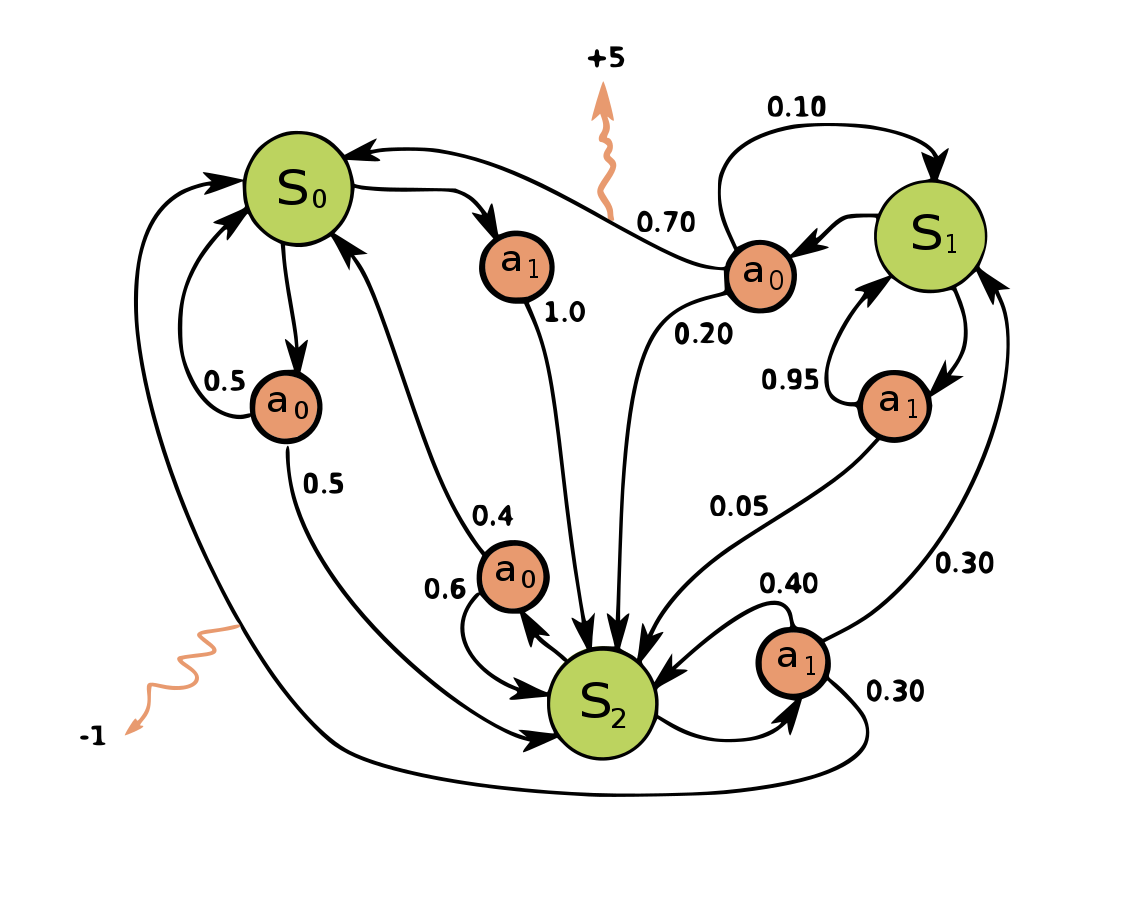
\includegraphics[scale=0.2]{Markov_Decision_Process.png}
\end{center}
	
To apply an algorithm to solve MDPs, two additional components are added. The first is the policy function $\pi$ which gives the probability for each potential action $a$ given the current state $s$. In some cases, such as with decision trees, this probability collapses to 1 for a particular action and 0 for all other actions. This function is what the algorithm seeks to approximate in the most optimal manner.

The second addition is $\gamma$, which is the discount factor. In the vast majority of cases, acting greedily is not the best move. For example, in a given game of chess, an opponent may sacrifice a valuable piece such as a rook in a gambit to take a queen. A greedy algorithm would always fall for this trap. When considering actions, we scan deeper into the MDP and sum future rewards as well. Since these future rewards are not guaranteed, the discount factor is multiplied with these values based on the ply, or depth of the search, to reduce its importance. Thus, the true goal the policy function $\pi$ seeks to optimize is

$$ R = \sum_{t=0}^{\infty} \gamma^t r_{a_t}(s_t,s_{t+1}).$$

MDPs are often represented as the tuple $(s, a, \pi, R, \gamma)$. $s$ is the set of all states. $a$ is the set of all actions. $\pi$ is the policy function that determines the probability of $a$ given $s$. $R$ is the reward function for transitioning from $s$ to $s'$. $\gamma$ is the discount factor for all future rewards considered. $\gamma \in [0,1]$, where $\gamma = 0$ means that the reward function ignores everything in the future (as $0^0=1$, but $0^t=0$, where $t>0$), and $\gamma = 1$ assumes perfect information, so the reward functions for all future states are weighted equally ($1^t=1$).

\subsection{Optimizing the Policy Function}

Original work in solving MDPs uses linear programming and dynamic programming. This is only applicable for very small MDPs that are fully computable such as tic-tac-toe. For all larger MDPs, a policy approximator must be used. Given the importance of creating decision making AI, a wide variety of approaches and algorithms have been developed over time preceding the rise of reinforcement learning.

The simplest and arguably most used method is through heuristics. When a policy function attempts to discern the optimal move, often the reward is unknown. For example, in chess a win would lead to a reward of 1 and a loss a reward of -1. This is obviously very distant from each individual move and prevents effective analysis of the state. This is called the credit assignment problem. Traditional approaches use heuristics to generate an evaluation of the board at each step. This intermediate value has the ability to evaluate the current state and determine its closeness to one of the end conditions.

A better heuristic results in more information and therefore a less noisy calculation of the reward. The primary problem can then be seen as generating a heuristic that best correlates with the true state of the board. Typically, these features are hand-crafted and identified by humans. While hand-crafted features have had far more success in this problem than other challenges like image perception as the number of features is smaller, there are still many cases in which these features are suboptimal or the problem is too complex for humans to be able to effectively represent all the features.
	
To account for this, machine learning is often introduced into decision making AIs to learn better heuristics. Typically, regression models such as random forests are used to estimate the reward. First, a model or a set of models are selected and trained on a specific task. The output of the trained model is used by the policy which simply picks the action with the maximum cumulative reward.
	
However, when using machine learning algorithms in this fashion, once again we see the rise of the credit assignment problem. This approach simply offloads the problem from the policy function to the model which learns the heuristic. In theory however, given enough data and effective regularization techniques combined with high batch sizes, the credit assignment problem can be somewhat dealt with. This system is sufficient enough to account for slightly more complex cases, namely in high level decisions where the set of actions is relatively small and states do not have large amounts of information. The truly big problems, such as teaching robots to walk, highly dimensional board games like Go, and quantitative stock analysis, are unsolvable.

\section{Reinforcement Learning}
To tackle these more pressing and valuable problems that are otherwise unaddressable, reinforcement learning (RL) is introduced. There are two primary components to reinforcement learning. The first is the policy, which has already been described. The second is the state-value function, which is more akin to heuristics and is how the reward is estimated.

\subsection{State-Value Function}
The primary task of the state-value function is to identify the optimal move at a given step. Recall that the cumulative reward function is defined as

$$ R = \sum_{t=0}^{\infty} \gamma^t r_{a_t}(s_t,s_{t+1}).$$

The first problem with this situation is the noisiness. The cumulative reward function is dependent on the original state and so optimizing it for one configuration does not ensure an optimal policy. The measurement of reward is dependent upon the initial situation, which induces error into the policy. Thus, the equation is modified to 

$$V_\pi = E[R] = E[\sum_{t=0}^{\infty} \gamma^t r_{a_t}(s_t,s_{t+1})]$$

where the expected reward over all possible initial states is maximized. To do this, data sampling must be done over a series of points sampled from the initial position distribution so that a variety of initial states are taken into account. Now, when $V$ is maximized, the learned policy is said to be the most optimal generalized policy. To further explore this, the equation is derived to

$$V_\pi(s) = \sum_a(s,a)\sum_{s'}P(s, a, s')[R(s, a) + \gamma V^\pi(s')].$$

This expresses the value of a state recursively as a function of the value of its previous state and is the Bellman equation. This is useful because $V_\pi$ is known to be the sole solution to its Bellman equation and it can be concluded this yields the optimal policy per the Bellman Principle of Optimality.

\subsection{Neural Networks}
The two components, the policy function and the state-value function, can then be modeled through neural networks. This allows us to use deep learning as a way to self-learn features. There are many ways neural networks model these functions and even more optimizers for each potential set up. These include Q-learning, SARSA, TD, DQN, dueling-DQN, and far more. This research uses trust region policy optimizers (TRPO), a more advanced version of proximal policy optimizers (PPO) which are generally considered to be the current best solution.

There are several changes made to traditional supervised learning that allow neural networks to be effectively applied to this type of problem. The most significant change is how data is accreted. Typical supervised learning requires annotated data which is fed into networks repeatedly over several epochs. For example, to train with supervised learning for chess, a database with thousands of games would be used and each move would be assigned a value based on the result of the game. The policy and state-value functions would subsequently be trained. 

However, as previously mentioned, the credit assignment problem makes training very noisy and demands massive batch sizes. In most cases, there isn’t enough data. To account for this, RL develops its own data through simulations. The current policy is run through a series of random starting environments several orders of magnitude higher than traditional batch sizes and these values are used to update the policy. For example, in the case of chess, the current policy would just play several thousand matches. This concept of learning from simulation is largely considered semi-supervised learning. The benefits of this mean that RL requires no data, the primary restriction mechanism in standard deep learning.

To run these simulations, an environment modeling the target problem is established. If RL was to be run on a board game, it would just self-play the matches needed. If RL was to be applied to a robot, an environment modeling physics would be created and thousands of attempts of it learning to move would be run. This concept ensures there is only one bound, computation time, as the limiting factor for this approach. It is also especially powerful for real world applications where data on the level needed for supervised learning cannot be acquired.

\subsection{Resource Demands}
Reinforcement Learning has shown itself to be the ultimate decision making algorithm, beating every standard and record set by both humans and computers in a vast array of problems. The progress it has made can help fundamentally change how AI make choices and address complex tasks. However, generalized usage of RL is still inhibited by the computational demands it requires. Given the sheer number of simulations and the massive batch sizes needed, very few organizations have the technical capabilities to apply RL. For example, it took Google 40+ days to fully train AlphaGoZero even when using 4 TPUs that provide a combined 720 teraflops of computing.

With such high requirements to run RL, mainstream usage has been fairly limited. This research aims to optimize reinforcement learning and accelerate the algorithm to allow for increased usage of this approach. This is primarily done through adversarial policies and dynamic environment manipulation.

\subsection{On Policy vs. Off Policy}
There are two major ways reinforcement learning learns policies. The primary problem in this area of AI is something called exploration vs. exploitation. This can be summarized as continuing to abuse the currently learned pattern for reward vs. exploring untouched regions of the state space for higher reward. There are many ways this problem is handled as it is rather common in CS, but for RL there are two major subfields that handle it differently.

The original approach for RL, Q learning, uses off policy optimization. Essentially, whenever a decision must be made in an MDP state, a greedy approach is used. This approach determines how we update our network and its values. This turns out to ensure we learn the optimal policy, however the proof is very extensive and not easily understood. 

The other approach is off policy optimizers. Off policy optimizers, like TRPO and PPO, use the currently learned policy to determine the action used to learn from. This means they follow the current thread more and do less exploration. As a result, they might not find the optimal policy. However, in practice this tends to be far faster as once the generally correct path is found, it can be searched farther faster. This turns out to be extremely useful because of the slowness of RL. 

To prevent over exploitation, off policy optimizers usually have some kind of noise parameter added in. However, because of the inherent noise in reinforcement learning and the sheer size of the state space in most problems, this isn't really a major issue. As a result, it is usually fine to use on policy optimizers and it is rare that using one causes significant performance decreases.

\subsection{Trust Region Policy Optimizer}
There are a wide variety of policy optimizers available for reinforcement learning. Most recently, proximal policy optimizers (PPO) have become standardized across the field as they have achieved comparable or superior results in nearly every type of task while being relatively simple to tune. PPO is an offshoot of TRPO which requires less parameter tuning and subsequently is easier to use for more problems. These are called on-policy optimizers.

The key property of interest in PPO and TRPO is proven convergence. This policy update procedure guarantees the policy will not diverge regardless of the initial state. This process is through the modified gradient calculation. In standard neural network backpropagation for supervised learning, the learning rate is a network-wide parameter that is independent of each specific weight. TRPO has a more complex approach to calculating the learning rate that makes it specific to each variable. This becomes very computationally expensive but is necessary to train reinforcement learning due to the instability.

The learning rate is established such that the change is within a specific trust region. This trust region is the area where we consider our policy to be a good approximation of the curve. This trust region is calculated using KL divergence between the original policy and the new policy we seek to update to. The difference between PPO and TRPO primarily comes in how this KL divergence is estimated because it is too computationally expensive to fully compute. Proximal policy optimizers only use first order optimization methods. However, TRPO implementations also uses the Fisher Information Matrix which is the second derivative of the KL divergence. This allows us to get a more accurate estimate of the trust region versus PPO.

This trust region technique of optimization, which is current standard practice, lends itself readily to the proposed acceleration through environment manipulation. When a policy is first trained in the simpler environment with less constraints, the trust region expands. This allows us to skip over local minima. Furthermore, the greater learning rate naturally lets us learn faster. By contrast, the smaller trust region from the more constrained environment leads to greater chance of falling into local minima and slower training.

\end{document}
